\section{Introduction} \label{sect:introduction}

The ``ChatGPT effect'' has taken the world by storm, and Large Language Models (LLMs) are now embedded in various applications that drive our daily lives. 
LLM-based AI agents elevate the applicability of LLMs through ``tool calling.'' Equipped with external tools, an LLM can \textit{interact} with its environment and autonomously execute tasks from start to finish, without further user intervention. As shown in \fig{fig:agent_overview}, given a user query (\circlednum{1}), the AI agent selects the appropriate tools to handle the request (\circlednum{2}). The agent then interacts with the environment (e.g., ``Contacts'', ``Calendar'', and ``Email'') by calling the selected tool (\circlednum{3}) and reflecting on prior tool output(s) to select the next action (\circlednum{4}). In academia, a rich body of prior work~\cite{react,reflexion,llmcompiler,lats} has improved agent task accuracy, while the industry has already started deploying LLM-based agents~\cite{deep_research,anthropic_agent,gemini_cli,chatgpt_agent,manus}, boosting user productivity and convenience.

On-device AI agents, which run entirely on a user’s local device, provide two unique benefits over cloud-based agents: availability and privacy. On-device agents are always available to the user for immediate use, regardless of the user's situation (lack of internet access) or the cloud provider's situation (server outage). Furthermore, growing concerns over data misuse call for measures to guarantee privacy in using LLMs, making on-device agents an attractive solution.

Building on this trend, various hardware and software have been introduced to ease the development and deployment of LLMs at the edge~\cite{copilot_pc,qualcomm_snapdragon_x_elite,amd_ryzen_ai_max,apple_m4_pro_max,qualcomm_snapdragon_hexagon_sdk,apple_foundation_models_framework}. Despite these advances, on-device AI agents still suffer from suboptimal latency, even for simple tasks, due to the resource-constrained nature of edge computing. Unlike cloud-based LLMs whose primary performance bottleneck lies in the decode stage, this paper makes the key observation that on-device agents spend a significant amount of time in \emph{both} the prefill and decode stages.  This key insight underscores the need for full-system acceleration techniques that address all key components of the agentic system pipeline on edge hardware.


\begin{figure}[t!] \centering
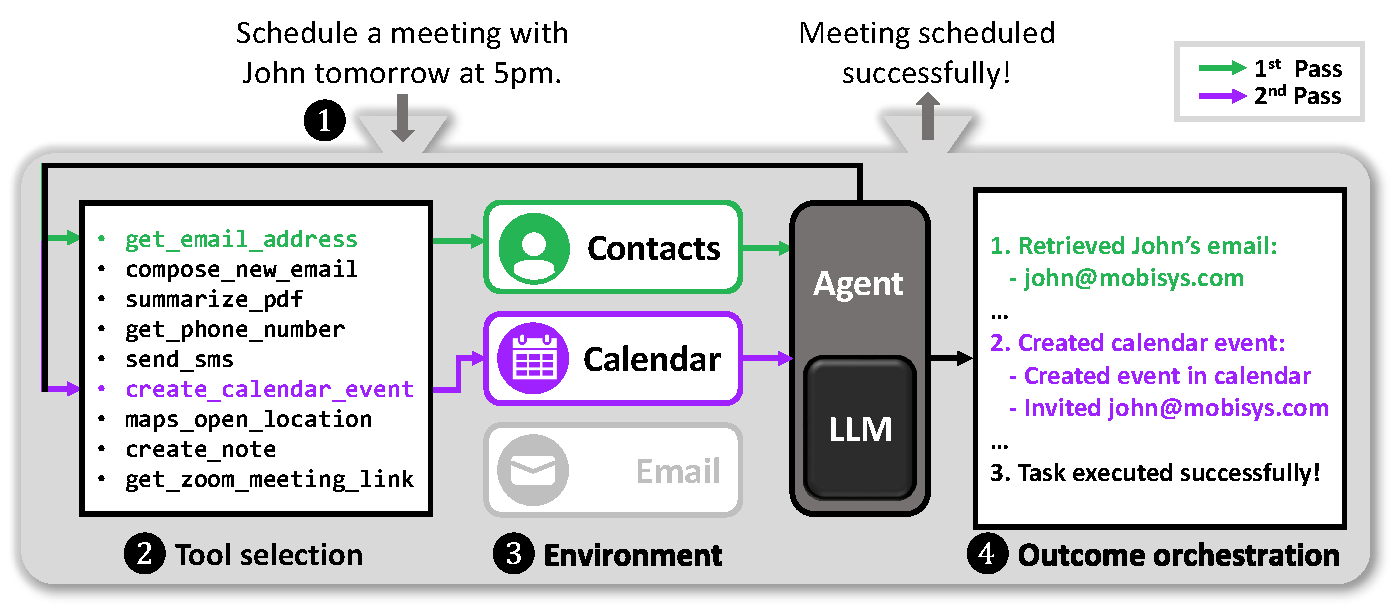
\includegraphics[width=\columnwidth]{./fig/agent_overview}
\caption{
Overview of an agentic system.
}
\Description{Overview of an agentic system.}
\label{fig:agent_overview}
\end{figure}


\begin{figure*}[t!] \centering
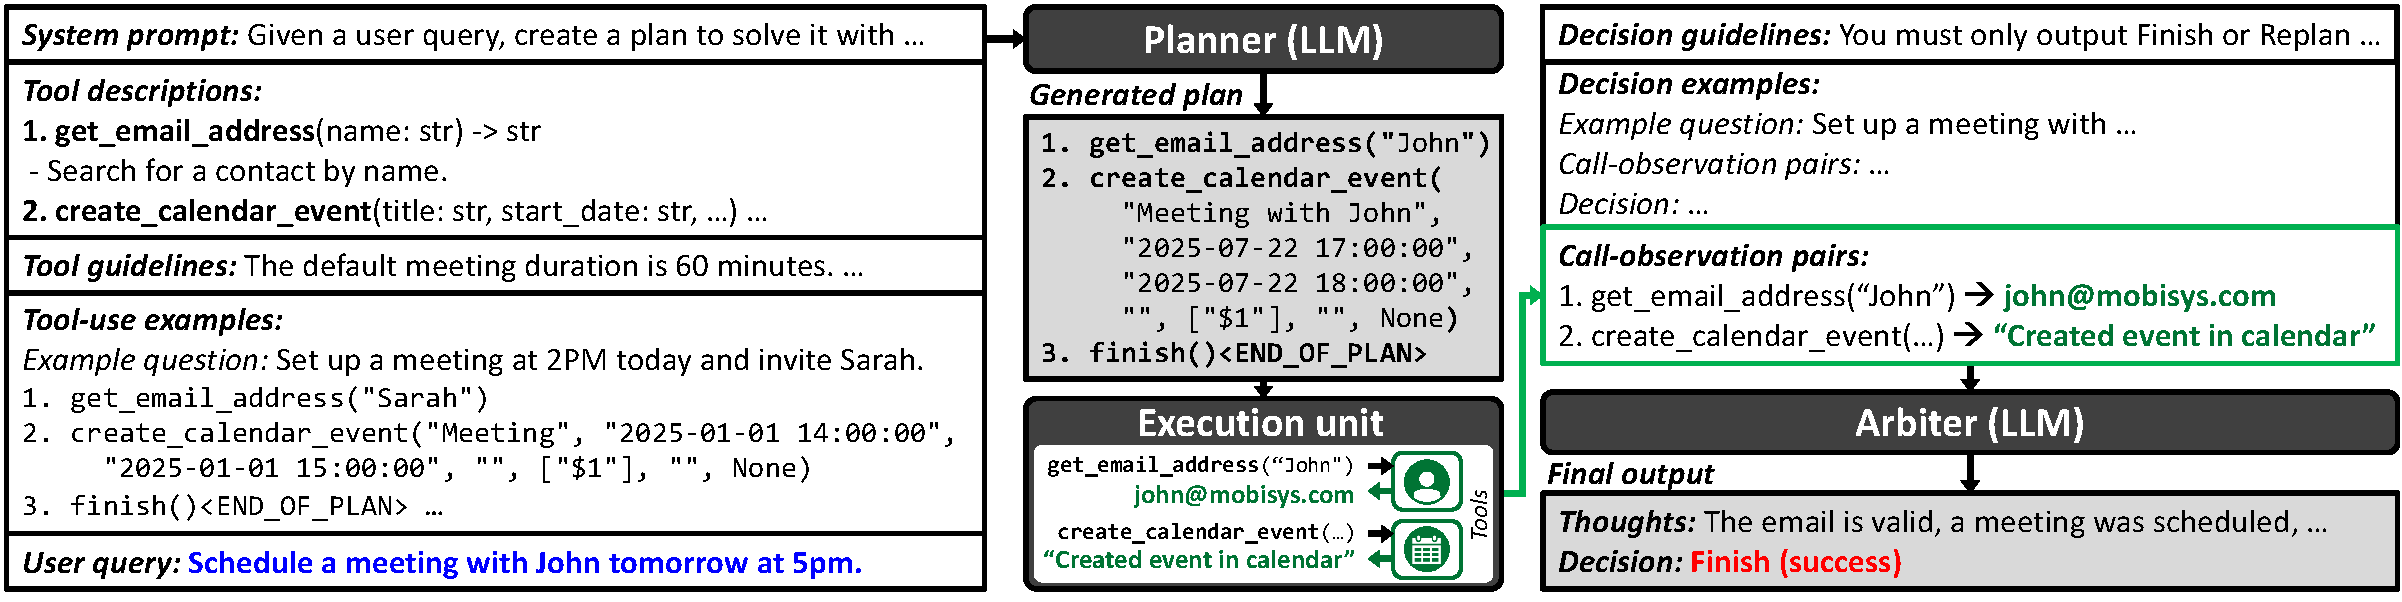
\includegraphics[width=1.0\textwidth]{./fig/plan-out_agents}
\caption{
Structure of plan-out agents. The whole pipeline consists of two LLMs (Planner and Arbiter) and a series of tool calls (carried out by Execution unit) to fully serve the user query (blue).
\Description{Structure of plan-out agents.}
}
\label{fig:plan-out_agents}
\end{figure*}


To this end, we propose \proposed, a purely software end-to-end acceleration scheme for on-device agents that does not degrade accuracy. To the best of our knowledge, this is the first work to provide a detailed system-level characterization of on-device AI agents. Building on this analysis, we introduce a full-pipeline acceleration solution that exploits both the algorithmic traits of agents and the hardware characteristics of edge environments, as detailed below.

{\bf On-device agents analysis.} We analyze the execution of LLM-based agents and identify two LLM instances as primary bottlenecks. Our analysis shows that, unlike conventional server-based, conversation-oriented applications where latency is dominated by decoding, both the prefill and decode stages contribute significantly to end-to-end latency in on-device environments due to the agentic workflow and hardware constraints. We further characterize these stages at the \textit{token level} and observe two key properties. First, during prefill, the prompt structure limits the applicability of optimizations such as prefix caching. Second, during decode, the output is largely grounded in few-shot examples and does not fully exploit the LLM’s reasoning capability.


{\bf Accuracy-preserving acceleration algorithm.} Building on our characterization, we propose \emph{\proposed}, which combines \emph{\prefill} and \emph{\decode} to accelerate the prefill and decode stages of on-device agentic LLMs, respectively. \prefill dynamically reconstructs the input prompt to enable efficient prefix caching, reducing online computation and substantially accelerating the prefill stage. We also note that, while speculative decoding~\cite{specdec, sps} is widely used to speed up LLM decoding, its reliance on additional LLMs hinders deployment on edge devices. To address this, \decode introduces a lightweight, prompt-aware draft model that enables efficient speculative decoding at the edge.


{\bf Real system integration.} We implement \proposed with Apple's MLX-LM~\cite{mlx_lm} and MLX-engine~\cite{mlx_engine}, and integrate it with TinyAgent~\cite{tinyagent} for a full system acceleration of on-device agents. Our evaluation shows that \prefill and \decode speed up the prefill and decode stages of on-device agentic LLMs by $1.97\times$ and $1.73\times$, respectively, achieving an average end-to-end task latency improvement of $1.61\times$.

Overall, \proposed accelerates on-device agents with minimal resource overhead. Its lightweight, accuracy-preserving, and purely software design allows direct integration into existing on-device agentic workflows, delivering immediate speedups and enabling fast, private agents at the edge.

